\documentclass[11pt,a4paper]{article}
\usepackage[margin=23mm]{geometry}
\usepackage[T1]{fontenc}
\usepackage{lmodern,microtype,amsmath,amssymb,graphicx,booktabs,tabularx,array}
\usepackage[authoryear,round,sort]{natbib}
\usepackage{xcolor,caption,fancyhdr,enumitem}
\usepackage[unicode,colorlinks=true,linkcolor=black,citecolor=black,urlcolor=teal]{hyperref}
\urlstyle{same}
\definecolor{teal}{HTML}{246C77}
\captionsetup{font=small,labelfont=bf,justification=raggedright,singlelinecheck=false}
\setlength{\parindent}{1.2em}
\setlength{\parskip}{2pt}
\setlength{\emergencystretch}{2em}
\linespread{1.00}
\setlength{\headheight}{14pt}
\pagestyle{fancy}\fancyhf{}
\fancyhead[L]{\small DSS5202 Sustainable Systems Analysis}
\fancyhead[R]{\small Group 04}
\fancyfoot[C]{\small\thepage}
\renewcommand{\headrulewidth}{0.3pt}
\newcommand{\co}{\ensuremath{\mathrm{kg\,CO_2e}}}
\newcommand{\note}[1]{\par\vspace{2pt}{\footnotesize\noindent\textit{Note.} #1\par}}
\newcolumntype{Y}{>{\raggedright\arraybackslash}X}
\newcommand{\page}{\clearpage}
\hypersetup{pdftitle={Buying New, Buying Second-Hand, or Renting?},pdfauthor={DSS5202 Group 04}}
\begin{document}
\thispagestyle{plain}
\begin{center}
{\LARGE\bfseries Buying New, Buying Second-Hand, or Renting?\par}
\vspace{6pt}
{\Large A Life-Cycle and AHP-Based Decision Analysis\\of Formalwear for Students\par}
\vspace{12pt}
{\normalsize Yang Yihua, Cao Xiaoyue, Yang Liu, Liu Ziqing, and Xie Tongling\par}
\end{center}
\vspace{2pt}
\begin{abstract}
Choosing formalwear involves environmental burdens, cash expenditure, and personal effort. This study compares buying one new dress, buying one second-hand dress, and renting the same model separately for six formal events attended by one student in one year. A screening life-cycle carbon assessment and consumer life-cycle costing model are combined with analytic hierarchy process (AHP) criteria weights and fixed-anchor performance scores. Manufacturing, distribution, and disposal are allocated by six annual wears relative to 26 assumed lifetime wears; purchase payments are charged in full. Calculated annual emissions are 4.9191 kg CO$_2$e for both purchases and 11.3797 kg CO$_2$e for rental. Annual expenditure is SGD 60.99 for second-hand, SGD 72.00 for new, and SGD 108.00 for rental. Second-hand ranks first (0.842087), followed by new (0.827428) and rental (0.529996). Rental collection and return travel explains most of its additional emissions and assumed active time. Only two of 17 complete individual AHP responses meet the consistency threshold, making the preference evidence exploratory. Results apply to the specified garment proxies, allocation rule, care arrangements, and travel assumptions; they do not establish a general advantage of ownership over rental.
\end{abstract}
\noindent\textit{Keywords:} formalwear; life-cycle assessment; consumer expenditure; second-hand clothing; analytic hierarchy process

\section{Introduction}
Students attending occasional formal events must decide whether to acquire a dress for repeated use or obtain temporary access through rental. A lower advertised rental fee need not imply a lower annual payment when each event requires a separate booking. Likewise, reuse does not by itself establish a smaller carbon footprint: garment lifetime, cleaning, and transport determine the burdens associated with providing the required service.

This report studies the Love, Bonito Eyka Multi-way Satin Column Dress in size S across three documented Singapore acquisition channels. It asks: \textit{For one student attending six formal events in one year, how do buying new, buying second-hand, and renting compare in allocated greenhouse gas emissions, direct expenditure, and an AHP-weighted decision score?} The alternatives provide the same model and permit repeated appearance. Their fit, suitability, hygiene, and availability are assumed adequate, rather than established by a physical inspection or six confirmed reservations.

The analysis follows a single chain from documented inputs to annual burdens, criteria weights, normalized scores, and interpretation. It evaluates three fixed alternatives. The resulting recommendation is conditional on the current model and evidence, with particular attention to the distinction between a quoted price, a literature proxy, a survey response, and a researcher assumption.

\page
\section{Background and Related Work}
\subsection{Clothing life cycles and access models}
Clothing comparisons require a common service basis. \citet{sandin2019} assess six garment types and document production and use inventories, including a polyester dress. Their reference garment supplies screening proxies, rather than measurements of the selected Eyka product.

Monticelli and Costamagna \citeyearpar{monticelli2023} compare formalwear rental with online purchasing in an Italian case. Their analysis separates life-cycle stages and shows why use frequency and service operations matter when interpreting rental. Their case uses a cotton dress and different ownership and rental lifetimes. Consequently, its comparative result is not transferred to the present alternatives; only the documented residential-care factor is used as a proxy. This report retains the existing project's common 26-wear lifetime across all channels, rather than introducing a rental lifetime advantage.

\subsection{AHP and performance scoring}
AHP structures decisions into a goal, criteria, and alternatives, using reciprocal pairwise judgments to derive priorities. \citet{saaty1994} discusses eigenvector priorities, geometric aggregation of group judgments, and consistency assessment. Here, AHP supplies weights for emissions, expenditure, and convenience. The alternatives' performances are evaluated using separately specified linear scores. This is an AHP-weighted scoring model: alternative priorities are not elicited through additional pairwise matrices.

\section{Study Design and Methodology}
\subsection{Functional unit, alternatives, and boundary}
The functional unit is suitable formalwear for one student attending six events in one year. Buying new and buying second-hand each involve one acquisition and six wears; rental involves six separate seven-day bookings, each covering one event. Events do not overlap, and outfit variety is not a requirement. Although the same product model is selected, the second-hand listing's colour is not confirmed to match the mint new and rental options.

The environmental boundary includes allocated manufacturing, pre-consumer distribution and retail, gross end-of-life disposal, annual cleaning, and acquisition-related delivery or passenger travel. The annual allocation includes a share of eventual disposal, without claiming that disposal occurs during the study year. The model excludes travel to the events, shoes and accessories, accidental repairs, and new packaging; existing packaging is assumed reused. No additional store, platform, or warehouse model is added to the retained distribution factor.

\begin{figure}[!htbp]
\centering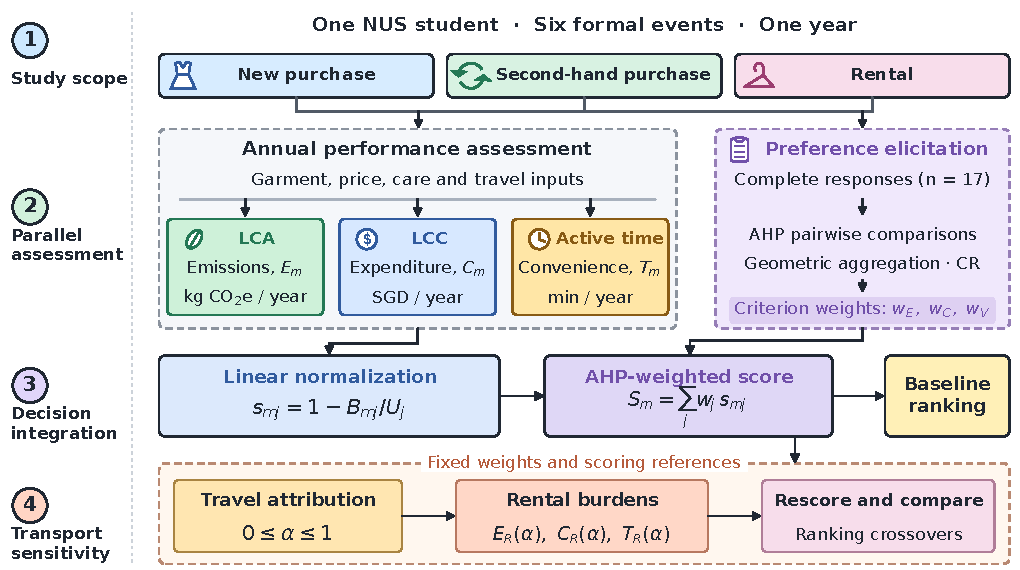
\includegraphics[width=\linewidth]{figures/framework.pdf}
\caption{Study workflow. Inputs retain separate evidence classes. Survey responses inform criteria weights; explicit assumptions enter burden and scoring calculations. Arrows indicate the analytical sequence.}
\label{fig:framework}
\end{figure}

\page
\subsection{Data sources and key assumptions}
Table~\ref{tab:inputs} distinguishes the four input classes. Market values are frozen advertised quotes recorded on 3 November 2026, not completed transactions. The official product page identifies a polyester main fabric and polyester--spandex lining, but actual item weight and fibre labels have not been independently checked \citep{lovebonito,usedquote,rentalquote}. The supplier instructs customers to wash before wearing. The rental listing instead asks users to return the dress without washing; the model therefore assigns cleaning after return.

\begin{table}[htbp]
\caption{Principal model inputs, evidence classes, and provenance.}
\label{tab:inputs}
\centering\small
\renewcommand{\arraystretch}{1.16}
\begin{tabularx}{\linewidth}{@{}>{\raggedright\arraybackslash}p{0.23\linewidth}>{\raggedright\arraybackslash}p{0.30\linewidth}Y@{}}
\toprule
Input & Retained value & Evidence class and source\\\midrule
Acquisition prices & New SGD 65; second-hand SGD 52; rental SGD 10/7 days & Original quotes: Love, Bonito; igotgr8deals; forest\_green66\\
Delivery and deposit & New SGD 0; second-hand SGD 1.99; rental refundable deposit SGD 99 & Original quote terms; full deposit refund is an assumption\\
Production / distribution / disposal & 14.8 / 0.84 / 0.99 \co\ per garment & Literature proxies, rounded from digitized Fig. 4.24 in Sandin et al. (2019); gross disposal, no energy credit\\
Reference garment & 0.478 kg polyester dress & Literature reference, not Eyka mass; no further mass multiplication\\
Cleaning emission factor & 0.109 \co\ per clean & Literature proxy: residential water-wash, drying and ironing, Monticelli and Costamagna (2023), Table 4\\
Rail / van factors & 0.0287 \co/passenger-km; 0.31844 \co/vehicle-km & UK 2026 proxies, direct plus energy upstream; DESNZ (2026)\\
Annual / lifetime use & 6 / 26 wears, all channels & Research scenario; lifetime informed by Sandin et al. (2019)\\
Cleaning activity & Purchases 7; rental 6 cleans/year & Research assumption: initial wash for purchases plus one after each wear\\
Transport activity & Purchases: $20/20=1$ vehicle-km each; rental: $6\times4\times10=240$ passenger-km & Assumed delivery route/batch and four dedicated rail legs per booking\\
Care / fares & SGD 1/home clean; SGD 2/travel leg; zero extra ordinary rental-care fee & Research assumptions, not service-provider confirmation\\
Convenience and anchors & 120 / 780 minutes; annual anchors 24 \co, SGD 360, 1080 minutes & Research assumptions; active time only\\
Criteria comparisons & Q8--Q10; 18 records, 17 complete & Original survey workbook; code-to-ratio mapping imposed by researchers\\
\bottomrule
\end{tabularx}
\note{DESNZ = Department for Energy Security and Net Zero. Full source locators and computational details are in Appendix~\ref{app:audit}. A recorded seller claim of one prior wear is not independently verified.}
\end{table}

The second-hand prior wear is used only to check remaining capacity: $1+6\leq26$. It does not change the allocation denominator to 25. No avoided-production credit or zero-production cut-off is assigned to second-hand. Local transport distances, batch size, fares, time, and rental care remain assumptions. The UK factors are used as transport proxies, rather than Singapore measurements \citep{desnz2026}.

\page
\subsection{Annual carbon accounting}
Let $m\in\{N,S,R\}$ denote new, second-hand, and rental, respectively. Let $n=6$ be annual wears, $L=26$ lifetime wears, and $M,D,F$ the per-garment manufacturing, distribution, and gross disposal factors. The screening LCA calculation is
\begin{equation}
 E_m=\frac{n}{L}(M+D+F)+k_m e_c+d_m e_v+p_m e_r ,
 \label{eq:lca}
\end{equation}
where $k_m$ is cleaning count, $e_c$ the cleaning factor, $d_m$ allocated delivery vehicle-kilometres, $e_v$ the van factor, $p_m$ passenger-kilometres, and $e_r$ the rail factor. Thus $(k_N,k_S,k_R)=(7,7,6)$, $(d_N,d_S,d_R)=(1,1,0)$, and $(p_N,p_S,p_R)=(0,0,240)$. Rental does not receive an additional purchase-delivery charge in the environmental calculation.

The common allocated garment burden is
\begin{equation}
 \frac{6}{26}(14.8+0.84+0.99)\approx3.8377\ \co\text{/year}.
\end{equation}
The 0.478 kg reference mass is descriptive only because the factors already refer to a garment. Applying it again would incorrectly scale the inventory. The retained disposal proxy represents gross collection and incineration emissions; an energy-recovery credit has not been deducted. Emissions are reported in kg CO$_2$e, using the source factors as supplied. Their geographical and impact-method differences limit harmonization, so this is a screening comparison rather than a product-specific verified footprint.

\subsection{Consumer life-cycle costing}
The LCC component is operationalized as one-year direct consumer expenditure in SGD. Let $P_m$ be purchase payment, $H_m$ delivery payment, $r_m$ rental fee per booking, $c_h$ home-care cost, $c_x$ extra rental-care fee, $b_m$ paid passenger legs, and $f$ fare per leg. Then
\begin{equation}
 C_m=P_m+H_m+n r_m+\mathbf{1}_{m\neq R}k_m c_h
       +\mathbf{1}_{m=R}n c_x+b_m f .
 \label{eq:lcc}
\end{equation}
Terms that do not apply to an alternative are zero. Both purchases incur their full acquisition payments, rather than $n/L$ of those payments. Manufacturing allocation distributes environmental service burdens across lifetime wears, whereas expenditure records the student's annual cash payments. These answer different accounting questions.

Resale receipts and year-end residual value are both set to zero. No discounting or monetization of time or emissions is applied. The SGD 99 refundable rental deposit is a temporary cash requirement, excluded from final net cost under the full-refund assumption. Sequential bookings do not require six simultaneously outstanding deposits. Normal return without damage or delay and no additional platform fees are assumed. Setting ordinary rental-care surcharges to zero is not evidence that cleaning is contractually included.

\subsection{Convenience as active consumer time}
The retained time proxy counts ordering, active home care, rental handling, and dedicated travel:
\begin{align}
 T_N=T_S&=15+7(15)=120\ \text{minutes/year},\\
 T_R&=6[10+4(30)]=780\ \text{minutes/year}.
\end{align}
These are researcher settings from the existing time configuration, not survey averages or timed observations. Passive machine operation and provider labour are excluded. Search and fitting are not separately measured. The proxy therefore captures only part of the broader convenience concept presented to respondents.

\page
\subsection{AHP elicitation, aggregation, and consistency}
The original workbook contains 18 response records. Q8--Q10 provide the three comparisons for emissions ($E$), cost ($C$), and convenience ($V$). One record, anonymously labelled R017, lacks Q8 and is excluded from complete matrices without imputation. The main analysis retains all 17 complete responses, including individually inconsistent matrices, to report the existing exploratory model transparently.

For Q8, codes 1 and 5 favour emissions and cost, respectively, with 3 indicating equal importance. The main researcher conversion assigns distance from the midpoint $|x-3|=0,1,2$ the intensities $1,3,5$. Hence the ratios for codes 1--5 are $(5,3,1,1/3,1/5)$ when code 1 favours the numerator. Q8 supplies $E/C$ and Q10 supplies $C/V$. For Q9, code 1 favours convenience, so its $E/V$ sequence is reversed. The questionnaire screenshot supplied by the authors confirms the endpoints: Q9 runs from ``strongly prefer convenience'' (1) to ``strongly prefer emissions'' (5); Q10 runs from ``strongly prefer cost'' (1) to ``strongly prefer convenience'' (5). Codes 2--4 have no separate verbal labels. Midpoint equality and symmetric intensity interpretation are researcher choices consistent with this scale layout, rather than explicitly labelled responses. These responses are not a directly elicited Saaty 1--9 scale.

For respondent $r$, the positive reciprocal judgment matrix is
\begin{equation}
 A^{(r)}=\begin{pmatrix}
 1&a_{EC}^{(r)}&a_{EV}^{(r)}\\
 1/a_{EC}^{(r)}&1&a_{CV}^{(r)}\\
 1/a_{EV}^{(r)}&1/a_{CV}^{(r)}&1
 \end{pmatrix}.
 \label{eq:matrix}
\end{equation}
The code obtains priorities using normalized row geometric means,
\begin{equation}
 g_i=\left(\prod_{j=1}^{3}a_{ij}\right)^{1/3},\qquad
 w_i=\frac{g_i}{\sum_{h=1}^{3}g_h}.
 \label{eq:weights}
\end{equation}
For a positive reciprocal $3\times3$ matrix this equals the principal eigenvector. The implementation also checks $Aw=\lambda_{\max}w$ numerically. Consistency is evaluated as
\begin{equation}
 \lambda_{\max}=\frac{1}{3}\sum_{i=1}^{3}\frac{(Aw)_i}{w_i},\qquad
 CI=\frac{\lambda_{\max}-3}{2},\qquad CR=\frac{CI}{0.52}.
 \label{eq:cr}
\end{equation}
The retained random index $RI=0.52$ comes from the $n=3$ table on printed page 104 of \citet{saaty1994}; $CR\leq0.10$ is the acceptance threshold. This specific source reports 0.52, rather than the 0.58 found in other RI tables.

For $q$ included respondents, judgments are aggregated with equal respondent weights before priorities are calculated:
\begin{equation}
 \bar a_{ij}=\left(\prod_{r=1}^{q}a_{ij}^{(r)}\right)^{1/q}.
 \label{eq:aggregate}
\end{equation}
Equation~\ref{eq:weights} and the consistency check are then applied to $\bar A$. Individual weight vectors are not arithmetically averaged. A second, already available result uses only respondents meeting the personal CR threshold under the same main mapping. It is reported as a descriptive comparison, without treating agreement in rank as a robustness validation. No new preference mapping or sensitivity experiment is introduced in this report.

\page
\section{Results}
\subsection{Annual emissions and their composition}
Figure~\ref{fig:emissions} shows the recalculated annual burdens. Both buying options produce 4.9191 \co/year, while rental produces 11.3797 \co/year. The purchased garments each combine 3.4154 for manufacturing, 0.1938 for distribution, 0.2285 for disposal, 0.7630 for cleaning, and 0.3184 for delivery. Their equality follows directly from identical lifetime allocation, cleaning counts, and delivery settings.

\begin{figure}[!htbp]
\centering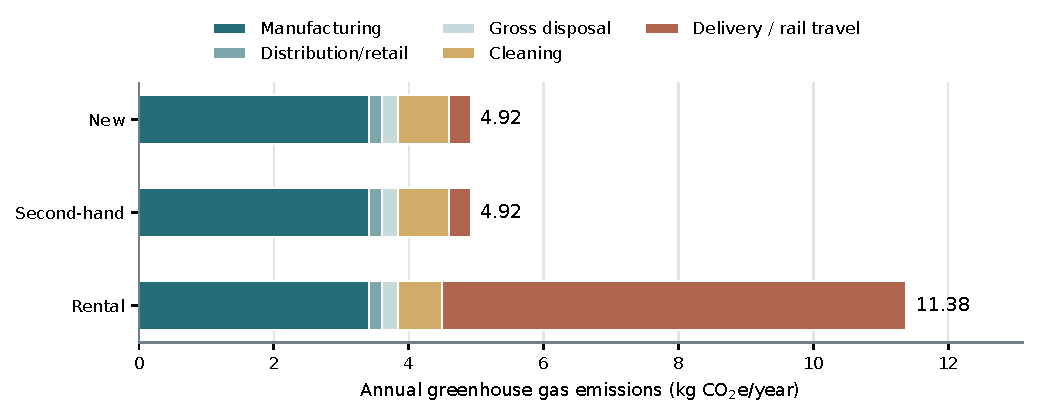
\includegraphics[width=.98\linewidth]{figures/emissions.pdf}
\caption{Annual greenhouse gas emissions by modelled life-cycle stage. Values are generated from \texttt{annual\_results.csv}; totals are rounded for display. Allocated garment stages use six of 26 lifetime wears for every option. Purchase delivery and rental passenger travel are shown together as the acquisition-transport stage.}
\label{fig:emissions}
\end{figure}

Rental has the same allocated garment stages, 0.6540 \co\ from six cleans, and 6.8880 \co\ from 240 passenger-kilometres. It exceeds either purchase by 6.4606 \co/year. Transport contributes an additional 6.5696, partly offset by 0.1090 less cleaning. Thus, under the retained travel arrangement, the additional burden is primarily associated with collection and return. It is not caused by a larger rental manufacturing allocation.

\subsection{Annual expenditure and its composition}
\begin{table}[htbp]
\caption{Consumer expenditure by component (SGD/year).}
\label{tab:cost}
\centering\small
\begin{tabular}{@{}ccccccc@{}}
\toprule
Option & Garment & Delivery & Rent & Care & Travel & Total \\
\midrule
New & 65.00 & 0.00 & 0.00 & 7.00 & 0.00 & 72.00 \\
Second-hand & 52.00 & 1.99 & 0.00 & 7.00 & 0.00 & 60.99 \\
Rental & 0.00 & 0.00 & 60.00 & 0.00 & 48.00 & 108.00 \\
\bottomrule
\end{tabular}

\note{Deposit is excluded from each total. The rental quote is SGD 10 per booking for six bookings; travel is 24 legs at an assumed SGD 2. Home care is seven cleans at an assumed SGD 1. Extra ordinary rental-care charges are assumed zero.}
\end{table}

Second-hand has the lowest annual expenditure at SGD 60.99, saving SGD 11.01 relative to new. Its SGD 13 lower garment price is partly offset by SGD 1.99 delivery. Rental's SGD 60 booking fees exceed the second-hand garment price and are supplemented by SGD 48 travel, giving SGD 108.00 annually. The refundable deposit remains relevant to liquidity even though it does not increase modelled final cost. Quoted rental penalties are not expected annual payments in the normal-return scenario.

\page
\subsection{Criteria weights and individual consistency}
Only 2 of 17 complete individual matrices (11.8\%) pass $CR\leq0.10$ under the main conversion. These are R006 and R015. Responses were not revised with respondents, and no personal judgment is described as consistent merely because it contributes to a consistent group matrix. Table~\ref{tab:ahp} reports the full-sample aggregate and the existing qualified subset.

\begin{table}[htbp]
\caption{Group AHP priorities under the retained main mapping.}
\label{tab:ahp}
\centering\small\begin{tabular}{@{}lrrrrr@{}}
\toprule
Sample & $n$ & $w_E$ & $w_C$ & $w_V$ & Group CR \\
\midrule
All complete & 17 & 0.200893 & 0.479329 & 0.319778 & 0.013001 \\
CR-qualified & 2 & 0.333333 & 0.333333 & 0.333333 & 0.000000 \\
\bottomrule
\end{tabular}

\note{The full-sample group has $\lambda_{\max}=3.013521$ and $CI=0.006760$. The qualified-subset aggregate is the all-ones matrix. A group CR below 0.10 does not resolve the 15 individual failures.}
\end{table}

Cost receives the largest full-sample weight (0.479329), followed by convenience (0.319778) and emissions (0.200893). The qualified two-person aggregate instead assigns one-third to each criterion. This substantial difference in weights limits any claim that the full-sample priorities are well-established student preferences.

\subsection{Normalization, scores, and ranking}
For burden $B_{mj}\in\{E_m,C_m,T_m\}$ and annual reference $U_j$, performance and composite scores are
\begin{equation}
 s_{mj}=1-\frac{B_{mj}}{U_j},\qquad
 S_m=w_Es_{mE}+w_Cs_{mC}+w_Vs_{mV}.
 \label{eq:score}
\end{equation}
The anchors are researcher settings: $U_E=6(4)=24$ \co/year, $U_C=6(60)=360$ SGD/year, and $U_V=6(180)=1080$ minutes/year. They are reference burdens for normalization, not observed maxima, spending constraints, or empirical acceptability thresholds. Scores are not clipped: a burden exceeding its anchor would yield a negative score. All current scores lie within the reference range. The scores are also not normalized to sum to one across alternatives.

\begin{table}[htbp]
\caption{Integrated annual results with full-sample AHP weights.}
\label{tab:ranking}
\centering\small\begin{tabular}{@{}lrrrrrrr@{}}
\toprule
Option & \co/year & SGD/year & Minutes & $s_E$ & $s_C$ & $s_V$ & $S$ (rank) \\
\midrule
Second-hand & 4.9191 & 60.99 & 120 & 0.7950 & 0.8306 & 0.8889 & 0.842087 (1) \\
New & 4.9191 & 72.00 & 120 & 0.7950 & 0.8000 & 0.8889 & 0.827428 (2) \\
Rental & 11.3797 & 108.00 & 780 & 0.5258 & 0.7000 & 0.2778 & 0.529996 (3) \\
\bottomrule
\end{tabular}

\note{E, C, and V scores refer to emissions, cost, and convenience. Annual emissions are displayed to four decimal places and composite scores to six; calculations retain full precision. Time values are assumed active minutes, not observations.}
\end{table}

Second-hand ranks first, followed by new and rental. The second-hand advantage over new is entirely the weighted cost-score difference, $0.479329(11.01/360)=0.014659$; their emissions and time scores are identical. Rental has lower performance scores on all three criteria under the current inputs.

Using only the two CR-qualified respondents gives scores of 0.838169 (second-hand), 0.827975 (new), and 0.501208 (rental), with the same order. This agreement describes two existing calculations. It does not validate robustness to uncertain lifetimes, service practices, score anchors, or survey coding, and no such validation is claimed.

\page
\section{Discussion and Limitations}
\subsection{Interpreting the comparison}
Buying second-hand combines the lowest annual payment with the same allocated emissions and active time as buying new. Rental's low single-booking price does not translate into a lower six-event cost. Four dedicated travel legs per booking add expenditure and effort; their emissions outweigh the single avoided clean.

Equal lifetime allocation is central to this interpretation. Rental receives no modelled benefit from achieving more lifetime uses than ownership, because every channel is assigned 26 wears. Second-hand is charged the same manufacturing share as new, even though the garment already exists. The comparison therefore concerns allocated burdens per annual service under a common rule; it does not estimate the marginal production avoided by a second-hand purchase or a rental transaction. Equality of new and second-hand emissions is a consequence of this model, not a general finding about these markets.

LCC charges the complete purchase price this year, while LCA assigns six wears' share of lifetime garment emissions. Annual affordability and environmental service attribution answer different questions. The purchase expenditure is therefore not a depreciated annual garment cost.

\subsection{Evidence and methodological limits}
First, the environmental results depend on proxy data. Production-related factors are rounded graphical extractions for a literature dress, not Eyka-specific measurements. The source's detailed and overview plots do not fully reconcile, and extraction precision is not measurement precision. Actual mass, construction, origin, and lifetime remain unverified. The residential cleaning proxy combines washing, drying, and ironing in an Italian setting; it does not measure local cold-water home care or the rental provider's actual process. UK transport factors are likewise not local rail or delivery intensities. Different source impact-method versions are retained without a common inventory recalculation.

Second, the market comparison is narrow and conditional. Advertised prices may change, and neither a transaction nor availability across all six dates was verified. The second-hand item's colour, delivered condition, and authenticity were not independently checked. Rental hygiene procedures, routine care charges, and extra platform fees remain unresolved. Assumed normal returns exclude damage and lateness costs, while zero resale and residual value omit possible retained financial value. These gaps limit generalization.

Third, the preference evidence is weak. Fifteen personal matrices fail the main CR threshold; low aggregate inconsistency can coexist with these failures. Unlabelled intermediate positions, the researcher-imposed intensity mapping, and the two-person qualified subset limit preference interpretation and generalization. Convenience is reduced to assumed active time, although the survey describes a broader mix of time and effort. Fixed score anchors establish implicit trade-off scales in addition to the AHP weights. No statistical representativeness, causal effect, or ranking robustness is established.

\section{Conclusion}
Under the retained six-event scenario, second-hand ranks first (0.842087), new second (0.827428), and rental third (0.529996). The purchase options each produce 4.9191 \co/year, compared with rental's 11.3797, while annual expenditures are SGD 60.99, SGD 72.00, and SGD 108.00, respectively. For a student able to rewear this model and use the assumed delivery and care arrangements, second-hand is the preferred option in the current calculation. This result is conditional on the shared 26-wear allocation, proxy factors, assumed travel and active time, and exploratory AHP evidence; it is not a universal recommendation.

\page
% APA 7 reference entries, maintained directly for a backend-independent build.
% natbib supplies author--year citations; all 3+ author citations use et al.
\begingroup
\small
\setlength{\bibsep}{9pt}
\begin{thebibliography}{99}
\raggedright

\bibitem[Aull-Hyde et~al.(2006)]{aullhyde2006}
Aull-Hyde, R., Erdogan, S., \& Duke, J. M. (2006). An experiment on the consistency of aggregated comparison matrices in AHP. \textit{European Journal of Operational Research, 171}(1), 290--295.
\url{https://doi.org/10.1016/j.ejor.2004.06.037}

\bibitem[Department for Energy Security and Net Zero(2026)]{desnz2026}
Department for Energy Security and Net Zero. (2026). \textit{Greenhouse gas reporting: Conversion factors 2026} [Data set and methodology]. GOV.UK.
\url{https://www.gov.uk/government/publications/greenhouse-gas-reporting-conversion-factors-2026}

\bibitem[Forman \& Peniwati(1998)]{forman1998}
Forman, E., \& Peniwati, K. (1998). Aggregating individual judgments and priorities with the analytic hierarchy process. \textit{European Journal of Operational Research, 108}(1), 165--169.
\url{https://doi.org/10.1016/S0377-2217(97)00244-0}

\bibitem[forest\_green66(n.d.)]{rentalquote}
forest\_green66. (n.d.). \textit{[For rent] LB Eyka multi-way satin column toga asymmetrical dress mint green} [Rental listing]. Carousell. Retrieved November 3, 2026, from
\url{https://www.carousell.sg/p/for-rent-lb-eyka-multi-way-satin-column-toga-asymmetrical-dress-mint-green-1464833759/}

\bibitem[igotgr8deals(n.d.)]{usedquote}
igotgr8deals. (n.d.). \textit{Eyka multi-way satin column dress} [Second-hand listing]. Carousell. Retrieved November 3, 2026, from
\url{https://www.carousell.sg/p/eyka-multi-way-satin-column-dress-1447640322/}

\bibitem[Love, Bonito(n.d.)]{lovebonito}
Love, Bonito. (n.d.). \textit{Eyka multi-way satin column dress} [Product page]. Retrieved November 3, 2026, from
\url{https://www.lovebonito.com/sg/eyka-multi-way-satin-column-dress-11k5111075.html}

\bibitem[Monticelli \& Costamagna(2023)]{monticelli2023}
Monticelli, A., \& Costamagna, M. (2023). Environmental assessment of the rental business model: A case study for formal wear. \textit{Environment, Development and Sustainability, 25}, 7625--7643.
\url{https://doi.org/10.1007/s10668-022-02363-x}

\bibitem[Saaty(1994)]{saaty1994}
Saaty, T. L. (1994). How to make a decision: The analytic hierarchy process. \textit{Atti del XXIV Incontro di Studio}, 75--105.
\url{https://doi.org/10.13128/Aestimum-7138}

\bibitem[Sandin et~al.(2019)]{sandin2019}
Sandin, G., Roos, S., Spak, B., Zamani, B., \& Peters, G. (2019). \textit{Environmental assessment of Swedish clothing consumption: Six garments, sustainable futures} (Mistra Future Fashion Report No. 2019:05). RISE Research Institutes of Sweden.
\url{https://research.chalmers.se/publication/514322/file/514322_Fulltext.pdf}

\end{thebibliography}
\noindent\textit{Bibliographic note.} Citation years follow the proceedings volume for Saaty (1994) and the journal volume for Monticelli and Costamagna (2023). Their online publication dates are June 1, 2009 and 2022, respectively. The original survey and analytical outputs are documented in Appendix~\ref{app:audit}.
\endgroup

\page
\appendix
\section{Source and Reproduction Notes}\label{app:audit}
\subsection{Source locators and evidence status}
The frozen market evidence is indexed as M2\_001 (official new product), M2\_002 (second-hand listing 1447640322), and M2\_003 (rental listing 1464833759) in \texttt{data/sources.json}; the brief extracts are in \texttt{evidence/market\_quotes.md}. The recorded access date is 3 November 2026, Singapore time. This report uses that frozen evidence and does not substitute a subsequently observed price. The rental listing's first-use deposit is SGD 99; a lower conditional deposit is not used in the baseline.

Environmental inputs are documented in \texttt{data/parameters.json} and \path{data/raw/literature_factors.csv}. The manufacturing, distribution, and disposal factors refer to printed page 83, Figure 4.24, of Sandin et al. (2019); the 0.478 kg reference is in Table B-59 on printed page 159. Figure extraction records are retained in \texttt{evidence/environment/}. The cleaning factor is the residential GWP entry in Table 4 of Monticelli and Costamagna (2023), printed page 7635; its washing inventory is in Table 2, page 7632. Only this care proxy is adopted, not the Italian study's full rental scenario.

The UK 2026 full-set workbook supplies rail/tram factors from \textit{Business travel--land} D89 and \textit{WTT--pass vehs \& travel--land} D86: $0.02121+0.00749=0.02870$ \co/passenger-km. Van factors use \textit{Delivery vehicles} D32 and \textit{WTT--delivery vehs \& freight} D31: $0.25716+0.06128=0.31844$ \co/vehicle-km. Selected cells and workbook hash are archived in \texttt{uk2026\_selected\_cells.json}. Transport upstream energy is included once; the gross disposal value is not replaced by a transport-only waste-reporting factor.

\subsection{Survey traceability and reporting scope}
The workbook \texttt{data/raw/survey\_18.xlsx}, sheet \textit{Original responses} (Chinese sheet name in the file), rows 2--19, columns J--L, supplies Q8--Q10. Question cells B27--B29 in the questions/rules sheet are transcribed in \texttt{results/run\_manifest.json}. The archived Q8 has five explicit labels. The author-supplied questionnaire screenshot verifies both Q9/Q10 endpoints: Q9 1 favours convenience and 5 emissions; Q10 1 favours cost and 5 convenience, with each endpoint labelled ``strongly prefer.'' Positions 2--4 are numbered without separate verbal labels. The model interprets 3 as equality and the two sides symmetrically; the 1/3/5 ratio mapping remains a researcher conversion, not an observed ratio scale. The question defines cost net of resale or retained value; the present zero-value settings make it numerically equal to expenditure.

Anonymous response IDs, source rows, ratios, personal weights, and CR values are available in \texttt{results/ahp\_individual.csv}. R017 is incomplete; R006 and R015 form the qualified subset under the main mapping. The report presents this mapping and its existing qualified subset only. Other diagnostics already produced by the project are not additional analyses undertaken for this paper.

\subsection{Reproduction and authorship}
Run \texttt{python code/run.py} from the project root, then regenerate report assets with \texttt{python report/generate\_assets.py}. The annual table and vector emissions chart read the resulting CSVs; no model parameters or questionnaire records are changed by the report scripts. Model checks use \texttt{python -m unittest discover -s tests -v}. Build instructions and the final verification record accompany the source.

Authors: Yang Yihua, Cao Xiaoyue, Yang Liu, Liu Ziqing, and Xie Tongling. Affiliation: Faculty of Science, National University of Singapore. Instructor: Kim Leng Poh.

\noindent\textit{AI use statement.} AI assistance was used for English drafting, LaTeX preparation, figure generation, and computational and document checks.
\end{document}
